% vim:set spell tw=79:

\documentclass[beamer]{uibk}
\title{Exploitation Techniques and Mitigations}
\subtitle{Dark Arts of Computer Science}
\author{Alex Hirsch \and Patrick Ober}
\date{2016-01-15}

\usepackage{multicol}
\newminted{nasm}{fontsize=\scriptsize,frame=leftline,framesep=2mm,linenos}

\AtBeginSection[] {
    \begin{frame}{Outline}
        \begin{multicols}{2}
            \tableofcontents[currentsection]
        \end{multicols}
    \end{frame}
}

\begin{document}

\maketitle

% \begin{frame}{Outline}
%     \begin{multicols}{2}
%         \tableofcontents
%     \end{multicols}
% \end{frame}

\begin{frame}{Acknowledgement}
    \begin{columns}
        \begin{column}{0.5\textwidth}
            We use a lot from RPISEC, a university course about modern
            exploitation at Rensselaer Polytechnic Institute (2015), because
            \dots

            \begin{description}
                \item<1->[of them:] They did a great job.
                \item<2->[of you:] You will see familiar material.
                \item<3->[of us:] We are lazy.
            \end{description}

            Check them out at \url{http://rpis.ec/} and
            \url{https://github.com/RPISEC/MBE}.
        \end{column}
        \begin{column}{0.5\textwidth}
            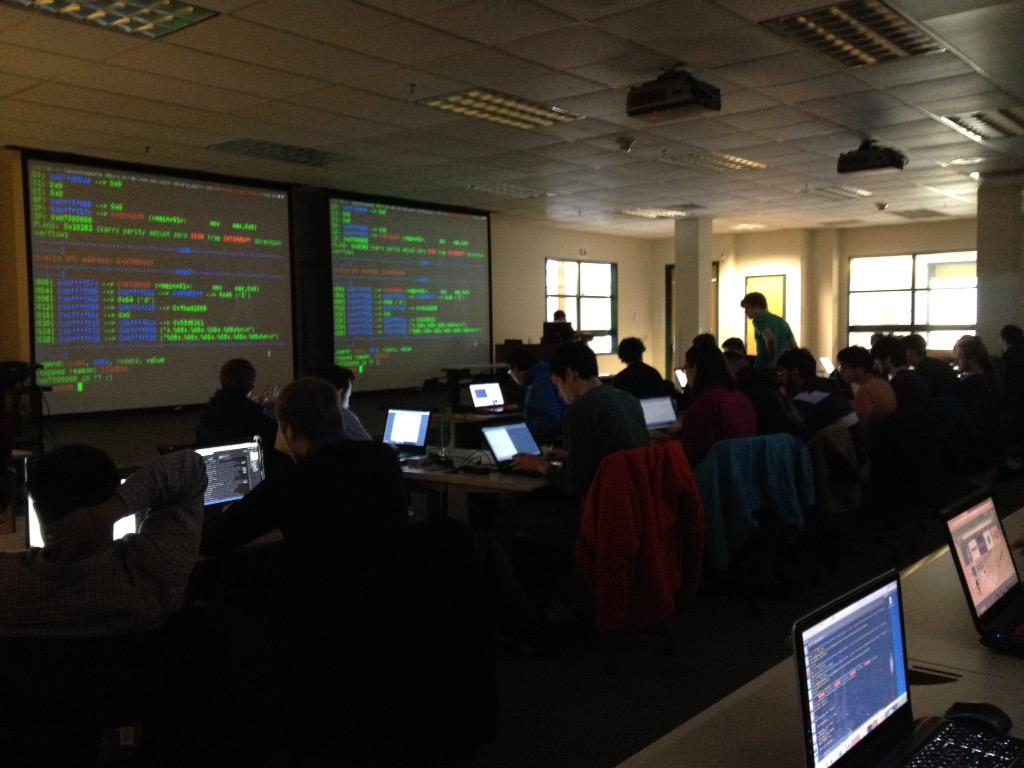
\includegraphics[height=0.7\textheight]{ripsec}
        \end{column}
    \end{columns}
\end{frame}

\section{Platform x86}

\begin{frame}{Why?}
    \begin{itemize}
        \item It's simpler, yet not overly simplified.
        \item Most techniques can be translated easily.
        \item Most material covers x86.
    \end{itemize}
\end{frame}

\begin{frame}{Registers}
    \begin{center}
        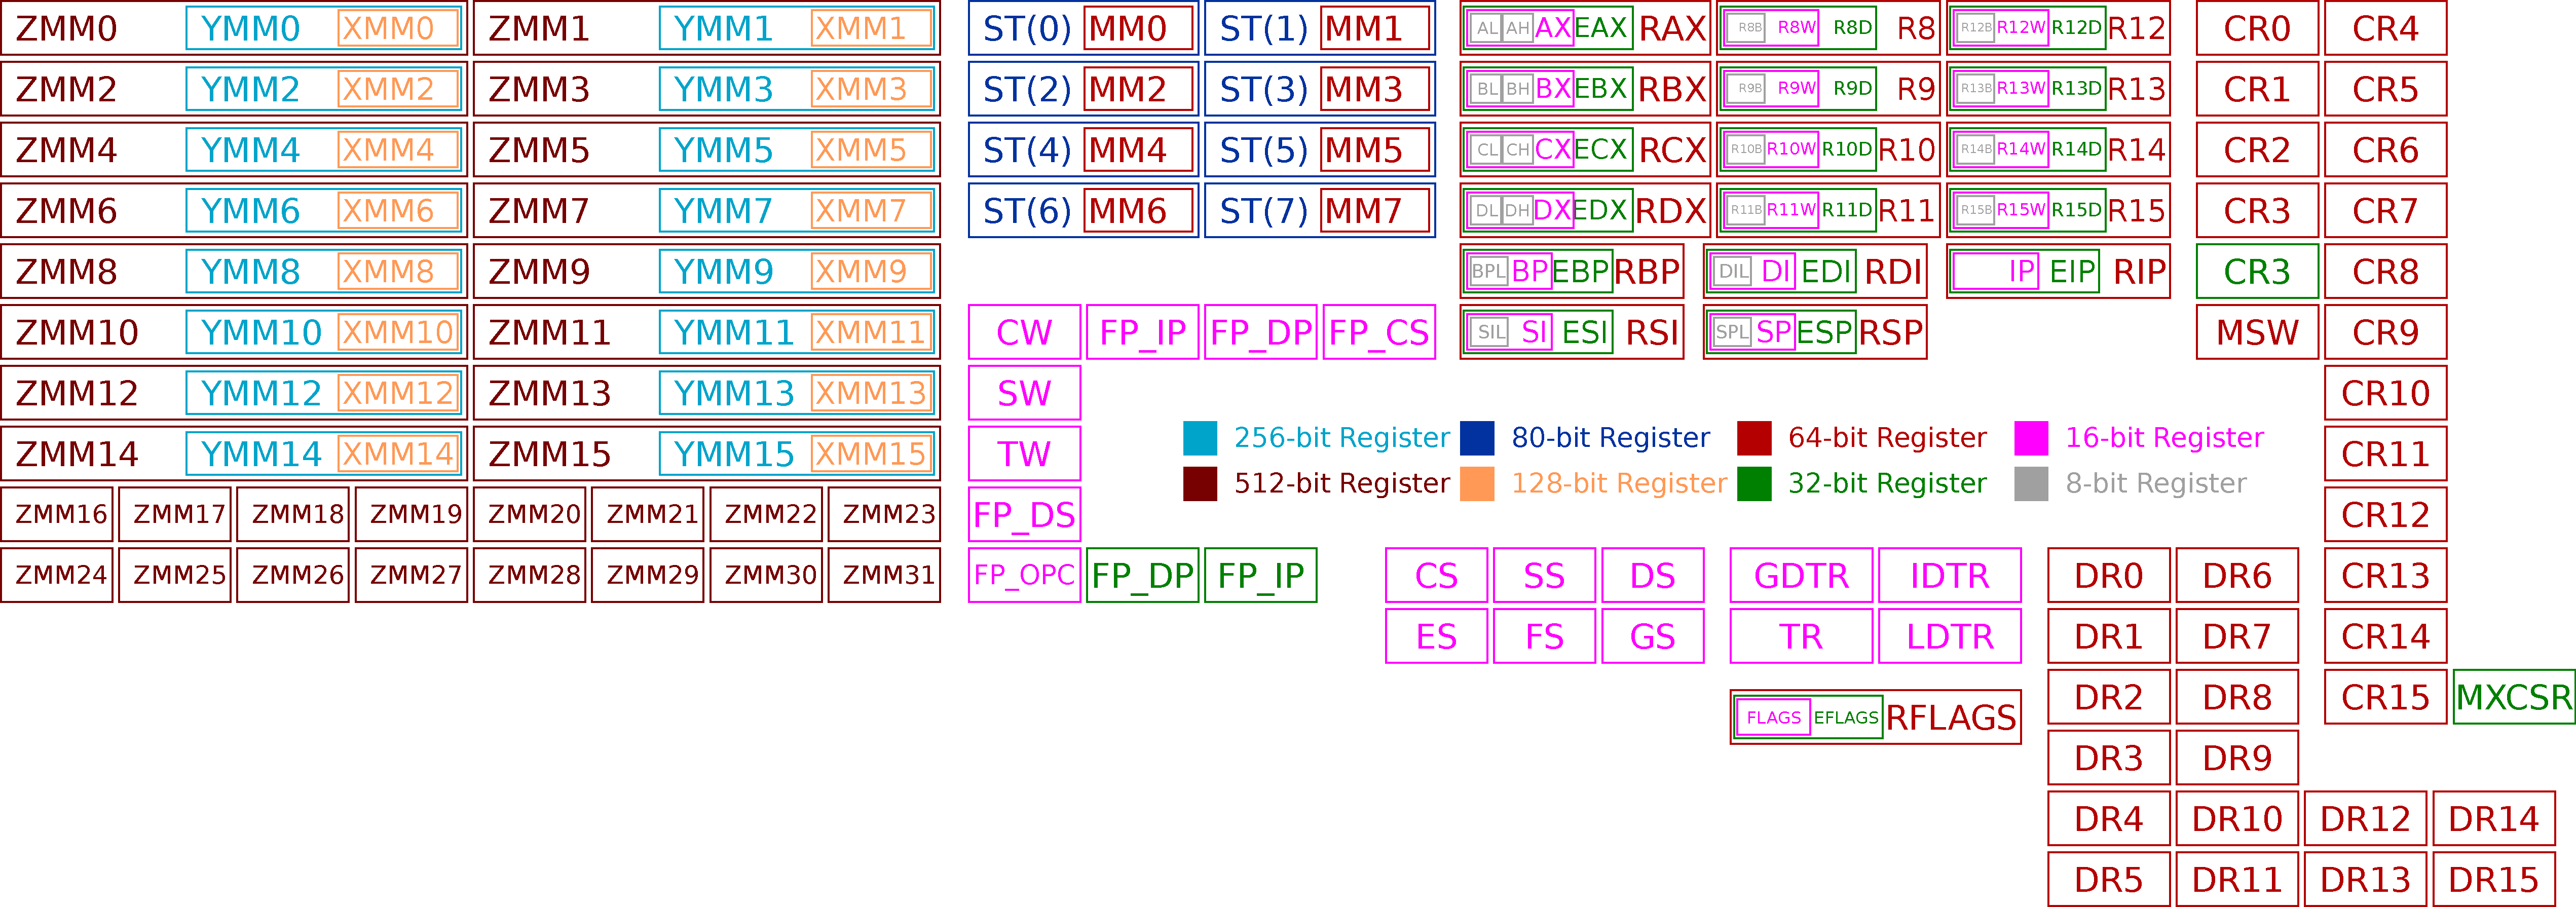
\includegraphics[width=\textwidth]{x86_registers}
    \end{center}
    \sidenote{- Wikipedia}
\end{frame}

\begin{frame}{Memory Management}
    \begin{columns}
        \begin{column}{0.45\textwidth}
            Real memory is managed by your OS kernel, a process sees only
            \textbf{virtual} memory.

            \medskip

            Memory is segmented (\textbf{pages}), which are handled by hardware
            (\textbf{memory management unit}) and software (kernel).

            \medskip

            \SI{4}{\kibi\byte} typical page size, addresses can be decomposed,
            page pointer + offset:

            $\mathtt{0xA1B2C3D4} \to \texttt{0xA1B2C000} + \mathtt{0x3D4}$
        \end{column}
        \begin{column}{0.55\textwidth}
            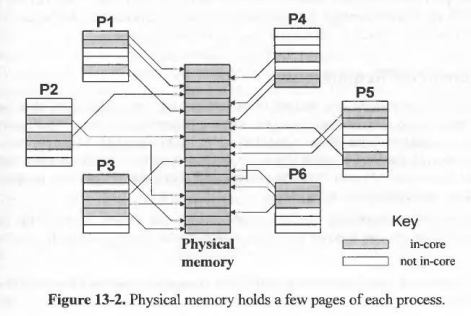
\includegraphics[height=0.7\textheight]{pages}
        \end{column}
    \end{columns}
    \sidenote{- Unix Internals by Uresh Vahalia}
\end{frame}

\begin{frame}{Process' Memory}
    \begin{columns}
        \begin{column}{0.5\textwidth}
            \begin{center}
                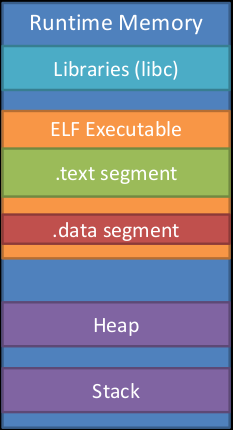
\includegraphics[height=0.8\textheight]{mem_layout}
            \end{center}
        \end{column}
        \begin{column}{0.5\textwidth}
            You know some of this, other talks also focus on this.

            \bigskip

            We'll see:
            \begin{itemize}
                \item Pages have permissions \texttt{rwx} (DEP)
                \item Layout not always the same (ALSR)
                \item Lots of pointers
            \end{itemize}
        \end{column}
    \end{columns}
\end{frame}

\begin{frame}{Calling Convention}
    \begin{columns}
        \begin{column}{0.5\textwidth}
            Defines:

            \begin{itemize}
                \item where to place arguments
                \item where to place return value
                \item where to place return address
                \item who prepares the stack
                \item who cleans afterwards\\
                    (caller vs.\ callee)
            \end{itemize}

            \pause

            Depends on:

            \begin{itemize}
                \item your platform
                \item your toolchain (language)
                \item your settings (compiler flags)
            \end{itemize}

        \end{column}

        \pause

        \begin{column}{0.5\textwidth}
            I know, Radu never told you\dots

            \medskip

            \textbf{C Declaration (cdecl):}

            \begin{itemize}
                \item arguments on stack (reverse order)\\
                    aligned to \SI{16}{\byte} boundary
                \item return via register (\texttt{EAX} / \texttt{ST0})
                \item return address on stack\\
                    (old instruction pointer \texttt{IP})
                \item old base pointer \texttt{BP}
            \end{itemize}
        \end{column}
    \end{columns}
\end{frame}

\begin{frame}[fragile]{System Call \& Protection Rings}
    \begin{columns}
        \begin{column}{0.55\textwidth}
            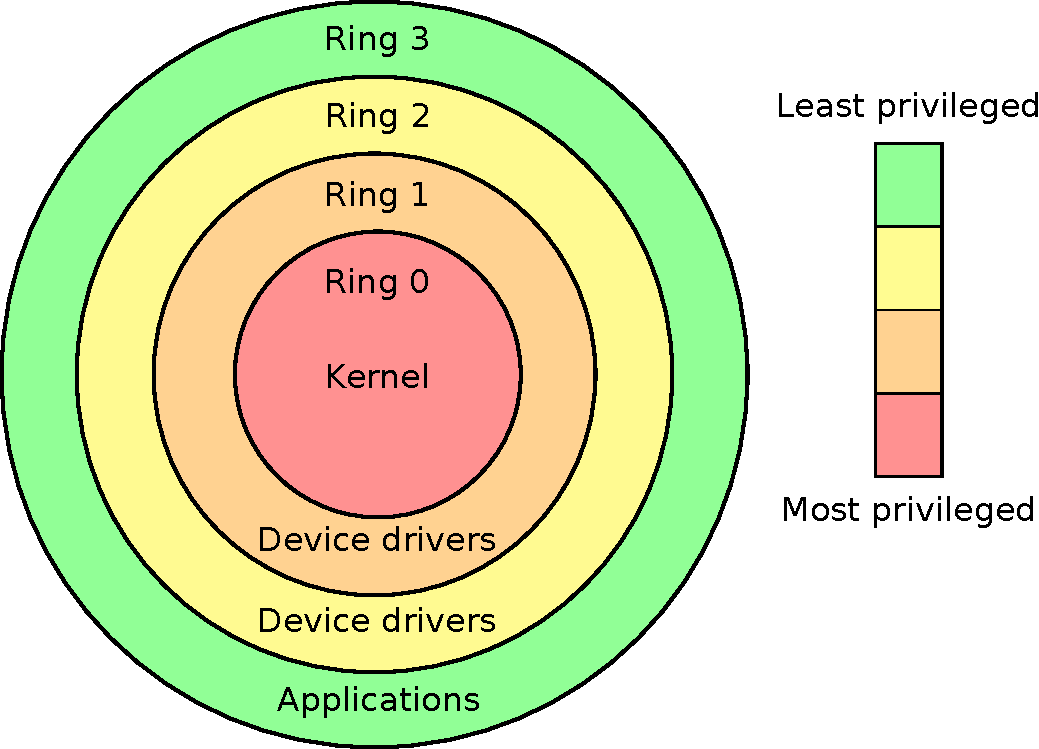
\includegraphics[width=\textwidth]{x86_rings}
        \end{column}
        \begin{column}{0.45\textwidth}
            Your CPU can switch from a more privileged state to a less
            privileged one.

            \bigskip

            Kernel does not run always, process cannot do everything (enforced
            by hardware).

            \bigskip

            Process uses a \emph{System Call} (own instruction) to notify the
            kernel to take over (context switch).

            \begin{nasmcode*}{autogobble,linenos=false}
                int   0x80   ; old
                call  write  ; new, sysenter via VDSO
            \end{nasmcode*}
        \end{column}
    \end{columns}
    \sidenote{- Wikipedia}
\end{frame}

\begin{frame}{System Calls}
    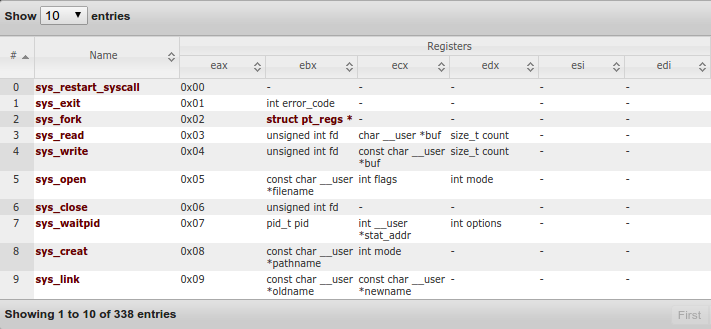
\includegraphics[width=\textwidth]{systemcalls}
    \sidenote{- \url{http://syscalls.kernelgrok.com/}}
\end{frame}

\begin{frame}{Endianness}
    \begin{columns}
        \begin{column}{0.5\textwidth}
            \begin{center}
                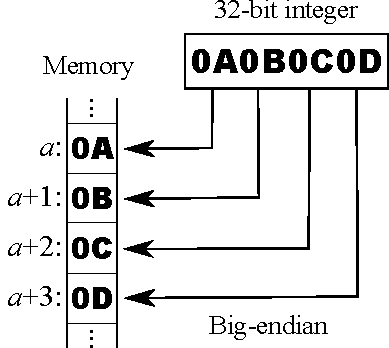
\includegraphics[width=0.8\textwidth]{big_endian}
            \end{center}
        \end{column}
        \begin{column}{0.5\textwidth}
            \begin{center}
                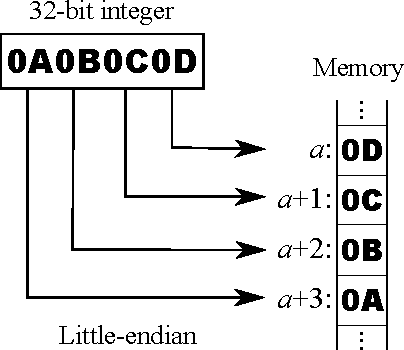
\includegraphics[width=0.8\textwidth]{little_endian}
            \end{center}
        \end{column}
    \end{columns}
    \sidenote{- Wikipedia}
\end{frame}

\section{Exploit printf}

\begin{frame}[fragile]{Death by \texttt{printf}}
    \begin{columns}
        \begin{column}{0.5\textwidth}
            \cfile[xleftmargin=0.8cm,firstline=4]{../format_string/main.c}
        \end{column}
        \begin{column}{0.5\textwidth}
            \pause
            \begin{pre*}{autogobble}
                ~> echo foobar | ./main
                You entered:
                foobar
            \end{pre*}
            \bigskip\pause
            \begin{pre*}{autogobble}
                ~> echo AAAABBBB | ./main
                correct
            \end{pre*}
            \bigskip\pause
            \begin{pre*} {autogobble}
                ~> echo '%08lx' | ./main
                You entered:
                7f380651f000
            \end{pre*}
            \medskip
            looks like a pointer, remember this for later.
        \end{column}
    \end{columns}
\end{frame}

\begin{frame}{Death by \texttt{printf}}
    \begin{center}
        \huge Demonstration
    \end{center}
\end{frame}

\section{Buffer Overflow}

\begin{frame}{Smashing the Stack}
    \begin{columns}
        \begin{column}{0.5\textwidth}
            \begin{center}
                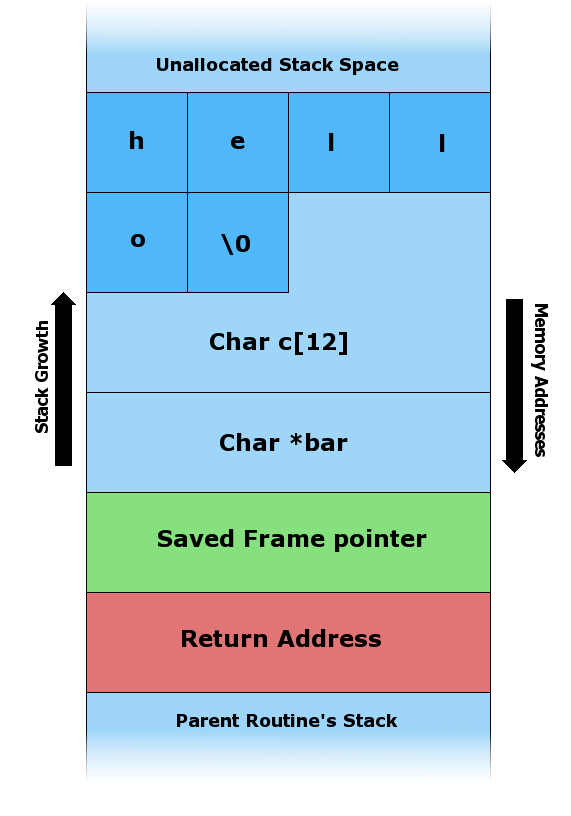
\includegraphics[width=0.75\textwidth]{stack_smash}
            \end{center}
        \end{column}
        \begin{column}{0.5\textwidth}
            \begin{itemize}
                \item Here, you write from top to bottom \bigskip
                \item You'll first overwrite local variables (\texttt{bar}) \bigskip
                \item Followed by arguments \bigskip
                \item Your \textbf{saved return address} \bigskip
                \item The next frame
            \end{itemize}
        \end{column}
    \end{columns}
    \sidenote{- Wikipedia}
\end{frame}

\begin{frame}[fragile]{Other variants}
    \begin{tabular}{p{0.5\textwidth} p{0.5\textwidth}}
        static memory corruption: &
        \begin{ccode*}{autogobble,linenos=false}
            static char buffer[64];
        \end{ccode*}
        \bigskip\\
        dynamic memory (heap) corruption: &
        \begin{ccode*}{autogobble,linenos=false}
            char *buffer = (char *) malloc(64);
            /* ... */
            free(buffer);
        \end{ccode*}
        \bigskip\\
        stack smashing: &
        \begin{ccode*}{autogobble,linenos=false}
            char buffer[64];
        \end{ccode*}
    \end{tabular}
\end{frame}

\begin{frame}{Overwrite a Flag}
    \begin{center}
        \huge Demonstration
    \end{center}
\end{frame}

\section{Shell Code}

\begin{frame}{Bend Return Address to jump into buffer}
    \begin{center}
        \huge Demonstration
    \end{center}
\end{frame}

\section{Data Execution Prevention (DEP)}

\begin{frame}{Data Execution Prevention}
    \begin{columns}
        \begin{column}{0.5\textwidth}
            \begin{center}
                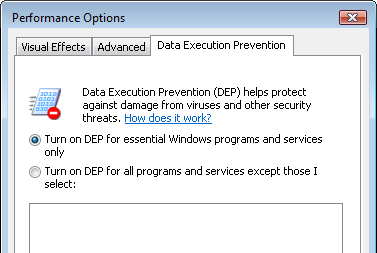
\includegraphics[width=0.9\textwidth]{dep_windows}
            \end{center}
        \end{column}
        \begin{column}{0.5\textwidth}
            \begin{itemize}
                \item also known as \textbf{write XOR execute} (\texttt{w\^{}x})
                \medskip
                \item sometimes called \textbf{page protection}
                \bigskip
                \item typically enforced by hardware
                \medskip
                \item \texttt{rwx} permissions per memory page
                \medskip
                \item \texttt{segfault} is triggered upon violation
            \end{itemize}
        \end{column}
    \end{columns}
\end{frame}

\begin{frame}{Data Execution Prevention}
    \begin{itemize}
        \item We cannot bend the return address to the buffer anymore
        \item What now?
        \pause
        \item Take control!
    \end{itemize}
\end{frame}

\begin{frame}{Return to a different function}
    \begin{center}
        \huge Demonstration
    \end{center}
\end{frame}

\section{Return Oriented Programming (ROP)}

\begin{frame}{Gadgets}

\end{frame}

\begin{frame}{Return to libC}

\end{frame}

\section{Address Space Layout Randomization (ASLR)}

\section{Heap Corruption}

\section{Stack Cookies}

\section{Code Pointer Integrity}

\section{ARM and x86\_64}

\section{Fuzzing}

\section{Polymorphic Code}

\section*{Conclusion}

\begin{frame}{Fin}
   \begin{center}
       \huge OMG finally\dots
   \end{center}
\end{frame}

\end{document}
